\documentclass[aps,preprint,nofootinbib,floatfix]{revtex4-1}
%\documentclass{article}

%\usepackage{nips_2017}

% to compile a camera-ready version, add the [final] option, e.g.:
%\usepackage[final]{nips_2017}

%\usepackage{nicefrac}       % compact symbols for 1/2, etc.
%\usepackage{microtype}      % microtypography
\usepackage{amsmath,amssymb,amsfonts,amsthm,amscd,bm,bbm}
%\usepackage{mathtools}
%\usepackage{printlen}
%\usepackage[inline]{enumitem}
%\usepackage{cite}
%\usepackage{bbm}

\usepackage[pdftex]{graphicx}
\graphicspath{{./figs/}}

\usepackage{algorithmic}
\usepackage{algorithm}

\hyphenation{op-tical net-works semi-conduc-tor}

\newtheorem{theorem}{Theorem}
\newtheorem{definition}[theorem]{Definition}
\newtheorem{assumption}[theorem]{Assumption}
\newtheorem{lemma}[theorem]{Lemma}
\newtheorem{corollary}[theorem]{Corollary}
\newtheorem{proposition}[theorem]{Proposition}
\newtheorem{conjecture}[theorem]{Conjecture}
\newtheorem{remark}[theorem]{Remark}
\newtheorem{example}{Example}

%% our definitions %%%%%%%%%%%%%%%%%%%%%%%%%%%%%%%%%%%%%%%%%%%%%%%%%%%%%%%%%%%%
\DeclareMathOperator{\aff}{aff}
\DeclareMathOperator{\st}{s.t.}
\DeclareMathOperator{\LC}{LC}
\DeclareMathOperator{\affnot}{aff_0}
\DeclareMathOperator{\conv}{conv}
\DeclareMathOperator{\relint}{relint}
\DeclareMathOperator{\vol}{vol}
\DeclareMathOperator{\range}{range}
\DeclareMathOperator{\image}{im}
\DeclareMathOperator{\nullspace}{null}
\DeclareMathOperator{\area}{area}
\DeclareMathOperator{\vspan}{span}
\DeclareMathOperator{\id}{Id}
\DeclareMathOperator{\cond}{cond}
\DeclareMathOperator{\prox}{prox}
\DeclareMathOperator*{\argmax}{arg\,max}
\DeclareMathOperator*{\argmin}{arg\,min}
\DeclareMathOperator*{\minimize}{minimize}
\DeclareMathOperator{\diag}{diag}
\DeclareMathOperator{\Tr}{Tr}

\newcommand\Energy{\mathcal{E}}
\newcommand\E{\mathbb{E}}
\newcommand\kk{K}
\newcommand\kkk{h}
\newcommand\Hk{{\mathcal{H}}_{\kk}}
\newcommand\HH{\mathcal{H}}
\newcommand\C{{\mathcal{C}}}
\newcommand\OO{{\mathcal{O}}}
%\newcommand\Zt{\widetilde{Z}}
\newcommand\Zt{Y}
%\newcommand{\Ind}[1]{\delta_{#1}}
\newcommand{\Ind}[1]{\mathbbm{1}_{#1}}


\begin{document}

\title{Nonparametric Clustering from  Energy Statistics}

\author{Guilherme Fran\c ca}
\email{guifranca@gmail.com} 
%\affiliation{Johns Hopkins University}

\author{Joshua T. Vogelstein}
\email{jovo@jhu.edu}

\affiliation{Johns Hopkins University}


\begin{abstract}
Energy statistics provides a nonparametric test for equality of distributions.
It was proposed by 
Sz\' ekely in the 80's,
inspired by Newton's potential energy between massive bodies. The idea
is to associate a statistical potential energy to observations such that 
minimum energy is achieved under the null hypothesis of equality of 
distributions. This 
was further generalized for probability 
distributions on arbitrary metric spaces,
and more recently, a connection with kernels in RKHS was established.
Nevertheless, although extensively used by the statistics community, it was
not incorporated in machine learning problems.
In this paper, we consider the problem of clustering data based
energy statistics theory. 
We provide a precise mathematical formulation, obtaining
a quadratically constrained quadratic optimization problem (QCQP). 
We show that
this is equivalent to kernel $k$-means
optimization problem, however,
energy statistics is able to fix the kernel choice. 
This method is nonparametric, and if prior information is available
it can be easily incorporated in the kernel construction.
We propose an algorithm
to find local optimizers of this QCQP problem based on the energy cost
of moving points to different clusters. We then compare this algorithm with
kernel $k$-means, standard $k$-means, and GMM. We test our method
on synthetic and real data experiments.
Our results show that energy statistics based clustering outperforms
these most used clustering algorithms.
\end{abstract}

\maketitle

\section{Introduction}

Mention why energy is important, main results, where it was applied, etc.
Motivate how this can be used for clustering. Mention most important
papers on this \ldots Explain main results of this paper and give a brief
outline.


%%%%%%%%%%%%%%%%%%%%%%%%%%%%%%%%%%%%%%%%%%%%%%%%%%%%%%%%%%%%%%%%%%%%%%%%%%%%%%%
\section{Background on Energy Statistics and RKHS}
\label{sec:background}

In this section we briefly review the main concepts from energy
statistics and its relation to reproducing kernel Hilbert spaces 
(RKHS) which form the basis of our work.
For more details we refer the reader
to \cite{Szkely2013} (and references therein) and 
also \cite{Sejdinovic2013}.

Consider random variables in $\mathbb{R}^D$ 
such that $X,X' \stackrel{iid}{\sim} P$ and 
$Y,Y' \stackrel{iid}{\sim} Q$, where $P$ and $Q$ are cumulative
distribution functions with finite first moments. 
The quantity \cite{Szkely2013}
\begin{equation}\label{eq:energy}
\Energy(P, Q) \equiv 2 \E \| X - Y\| - \E \| X - X' \| - \E \| Y - Y' \|,
\end{equation}
called \emph{energy distance}, 
is rotational invariant and nonnegative, $\Energy(P,Q) \ge 0$, where
equality
to zero holds if and only if $P = Q$.
Above $\| \cdot \|$ denotes the
Euclidean norm in $\mathbb{R}^D$. 
Energy distance
provides a characterization of equality of distributions and
$\Energy^{1/2}$ is
a metric on the space of distributions.

The energy distance can be generalized as, for instance,
\begin{equation}\label{eq:energy2}
\Energy_\alpha(P, Q) \equiv 
2 \E \| X - Y\|^{\alpha} - \E \| X - X' \|^{\alpha} - 
\E \| Y - Y' \|^{\alpha},
\end{equation}
where $0<\alpha\le 2$. This quantity is also nonnegative,
$\Energy_\alpha(P,Q) \ge 0$. Furthermore, for $0<\alpha<2$ we have 
$\Energy_\alpha(P,Q) = 0$ if and only if $P=Q$, while for $\alpha=2$ 
we have $\Energy_2(P,Q) = 2\| \E(X) - \E(Y) \|^2$ showing that
equality to zero only requires
equality of the means and thus $\Energy_2(P,Q)=0$ does 
not imply equality of distributions.

It is important to 
mention that \eqref{eq:energy2} can be even further generalized.
Let $X, Y \in \mathcal{X}$,  where $\mathcal{X}$ is a space endowed
with a \emph{semimetric of negative type}
$\rho: \mathcal{X}\times\mathcal{X} \to \mathbb{R}$, which satisfies
\begin{equation}
\label{eq:negative_type}
\sum_{i,j=1}^n \alpha_i \alpha_j \rho(X_i, X_j) \le 0,
\end{equation}
where $X_i \in \mathcal{X}$ and $\alpha_i \in \mathbb{R}$ such that
$\sum_{i=1}^n \alpha_i = 0$. Then $\mathcal{X}$ is called a space of
negative type.
We can thus replace $\mathbb{R}^D \to \mathcal{X}$ and 
$\| X - Y \| \to \rho(X , Y)$ in the definition \eqref{eq:energy} obtaining
the energy distance as
\begin{equation}\label{eq:energy3}
\Energy(P, Q) \equiv 2 \E \rho(X,Y) - \E \rho(X, X') - \E \rho(Y,Y').
\end{equation}
For spaces of negative type exists a Hilbert space $\mathcal{H}$ and
a map $\varphi: \mathcal{X} \to
\mathcal{H}$ such that
$\rho(X, Y) = \| \varphi(X) - \varphi(Y) \|_{\mathcal{H}}^2$. 
Even though the semimetric 
$\rho$ may not satisfy the triangle inequality, 
$\rho^{1/2}$ does since it can be shown to be a legit metric. 

There is an equivalence between energy distance, 
commonly used in statistics,
and distances between embeddings of distributions in 
RKHS, commonly used in machine learning. 
This equivalence was established
in \cite{Sejdinovic2013}. We first recall the definition of
RKHS. Let $\HH$ be a Hilbert space of real-valued functions
over $\mathcal{X}$. A function 
$\kk : \mathcal{X} \times \mathcal{X} \to 
\mathbb{R}$ is a reproducing kernel of $\HH$ if it satisfies
the following two conditions:
\begin{enumerate}
\item $\kkk_x \equiv \kk(\cdot, x) \in \HH$ 
for all $x \in \mathcal{X}$.
\item $\langle \kkk_x, f \rangle_{\HH} = f(x)$ for
all $x\in\mathcal{X}$ and $f\in \HH$.
\end{enumerate}
In other words, for any $x \in \mathcal{X}$ and any function $f \in \HH$ 
there is a unique 
$\kkk_x \in \HH$ that reproduces $f(x)$ through the inner product
of $\HH$.
If such a \emph{kernel} 
function $\kk$ exists then $\HH$ is called a RKHS. The above two 
properties immediately imply that $\kk$ is symmetric and positive
definite. Indeed, notice that
$\langle \kkk_x, \kkk_y \rangle = \kkk_y(x) = \kk(x,y)$, and since
this inner product is real,
$\langle \kkk_x, \kkk_y \rangle^* = \langle \kkk_y, \kkk_x \rangle = 
\langle \kkk_x, \kkk_y \rangle$, we immediately have that
the kernel is symmetric,
$\kk(y,x) = \kk(y,x)$. Moreover, for any $w \in
\HH$ we can write $w = \sum_{i=1}^n c_i \kkk_{x_i}$, where
$\{ \kkk_{x_i} \}_{i=1}^n$ is a basis of $\HH$. It follows that
$\langle w, w \rangle_{\HH}  = \sum_{i,j=1}^n c_i c_j \kk(x_i,x_j) \ge 0$
showing that the kernel is positive definite. If $G$ is a matrix with
elements $G_{ij} = \kk(x_i,x_j)$, this is equivalent to $G$ being
positive semi-definite, $\bm{w}^\top G \bm{w} \ge 0$ for any vector
$\bm{w} \in \mathbb{R}^n$.

The Moore-Aronszajn theorem establishes the converse \cite{Aronszajn}.
For every symmetric
and positive definite function $\kk: \mathcal{X}\times \mathcal{X} \to
\mathbb{R}$, there is an associated RKHS $\Hk$ 
with reproducing
kernel $\kk$. The map $\varphi: x \mapsto \kkk_x \in \Hk$ is called
the canonical feature map. Given a kernel $\kk$,
this theorem enables us to define an embedding of a probability measure
$P$ into the RKHS: $P \mapsto \kkk_P \in
\Hk$ such that 
$\int f(x) d P(x) = \langle f, \kkk_P \rangle$ for all $f \in \Hk$,
or alternatively, $\kkk_P = \int \kk( \, \cdot \,, x)  d P(x)$. 
We can now  introduce the 
notion of distance between two probability measures using the inner product
of $\Hk$. This is called the maximum mean discrepancy (MMD) and
is given by
\begin{equation}\label{eq:mmd}
\gamma_\kk(P,Q) \equiv \| \kkk_P - \kkk_Q \|_{\Hk},
\end{equation}
which can also be written as \cite{Gretton2012}
\begin{equation}\label{eq:mmd2}
\gamma_\kk^2(P,Q) = \E \kk(X,X') + \E \kk(Y,Y') - 2 \E \kk(X, Y)
\end{equation}
where $X,X' \stackrel{iid}{\sim} P$ and $Y,Y'\stackrel{iid}{\sim} Q$.
From the equality between \eqref{eq:mmd} and \eqref{eq:mmd2} we also
have 
\begin{equation}\label{eq:inner_data}
\langle \kkk_P, \kkk_Q \rangle_{\Hk} = \E \, \kk(X, Y).
\end{equation}
Therefore, in practice, we can estimate the inner product between the 
embedded distributions 
by averaging the kernel function over sampled data.

The following important result shows that semimetrics of negative
type and symmetric positive semidefinite kernels are closely related
\cite{Berg1984}. Let $\rho: \mathcal{X} \times \mathcal{X} \to \mathbb{R}$,
and $x_0 \in \mathcal{X}$ an arbitrary but fixed point.
Define
\begin{equation}
\label{eq:kernel_semimetric}
\kk(x,y) = \tfrac{1}{2} \left\{  \rho(x,x_0) + \rho(y,x_0) - \rho(x,y)\right\}.
\end{equation}
Thus, $\kk$ is positive semidefinite if and only if $\rho$ is a semimetric
of negative type
\eqref{eq:negative_type}.
Here we have a family of kernels, one for each choice of $x_0$. Conversely,
if $\rho$ is a semimetric of negative type and $\kk$ is a kernel in this
family, then 
\begin{equation}
\label{eq:gen_kernel}
\begin{split}
\rho(x,y) &= \kk(x,x) + \kk(y,y) -2\kk(x,y) \\
&=  \| \kkk_x - \kkk_y \|^2_{\Hk},
\end{split}
\end{equation}
and the canonical feature map 
$\varphi: x \mapsto \kkk_x$ is injective \cite{Sejdinovic2013}.
We say that the kernel $\kk$ generates the semimetric $\rho$. 
If two different kernels generate the same $\rho$ they are
equivalent kernels.

Now we can state the equivalence between energy distance $\Energy$ and
inner products on RKHS, which is one of the main results of
\cite{Sejdinovic2013}. If $\rho$ is a semimetric
of negative type and $\kk$ a kernel that generates $\rho$, then
replacing \eqref{eq:gen_kernel} into
\eqref{eq:energy3} and using \eqref{eq:mmd2} yields
\begin{equation} \label{eq:Erho}
\Energy(P, Q) = 
2 \left[ \E \, \kk(X, X') + \E \, \kk(Y, Y') - 2\E \, \kk(X, Y)\right] 
= 2 \gamma_\kk^2(P,Q) .
\end{equation}
Since $\gamma_k^2(P, Q) = \| \kkk_P - \kkk_Q \|^2_{\Hk}$ we
can compute the energy distance using the inner product of $\Hk$. Moreover,
this can be computed from the data according to \eqref{eq:inner_data}.

Finally, let us recall the main formulas for test statistics
of equality of distributions \cite{Szkely2013}. 
Assume we have data $\mathbb{X} = \{ x_1,\dotsc, x_n \}$, where
$x_i \in \mathcal{X}$ and $\mathcal{X}$ is a space of negative type.
Consider a partition $\mathbb{X} = \bigcup_{j=1}^k \C_j$, with
$\C_i \cap \C_j = \emptyset$.
Each expectation in 
\eqref{eq:energy3}
can be computed 
through the function
\begin{equation}
\label{eq:g_def}
g (\C_i, \C_j) \equiv 
\dfrac{1}{n_i n_j}
\sum_{x \in \C_i} 
\sum_{y \in \C_j} \rho(x, y)
\end{equation}
where $n_i = |\C_i|$ is the number of elements in 
$\C_i$. 
The \emph{within energy dispersion} is defined by
\begin{equation}
\label{eq:within}
W \equiv
\sum_{j=1}^{k} \dfrac{n_j}{2} g(\C_j, \C_j),
\end{equation}
and the \emph{between-sample energy statistic} is defined by
\begin{equation}
\label{eq:between}
S \equiv
\sum_{1 \le  i < j \le k } \dfrac{n_i n_{j}}{2 n} \left[
2 g(\C_i, \C_j) - 
g(\C_i, \C_i) - 
g(\C_j, \C_j)
\right].
\end{equation}
Given a set of distributions
$\{ P_j\}_{j=1}^k$, where $x \in \C_j$ if and only if $x \sim P_j$, 
the quantity $S$ provides
a \emph{nonparametric} test statistic for equality of distributions
\cite{Szkely2013}.
When the sample size is large enough, $n\to \infty$,
under the null hypothesis $H_0: P_1=P_2=\dotsm=P_k$ we have that
$S\to 0$, 
and under
the alternative hypothesis $H_1: P_i \ne P_j$ for at least two $i\ne j$, 
we have that $S \to \infty$.
This test is nonparametric in the sense that it does not make any assumptions
about the distributions $P_j$. Next we show how we can use $S$ for clustering
data.


%%%%%%%%%%%%%%%%%%%%%%%%%%%%%%%%%%%%%%%%%%%%%%%%%%%%%%%%%%%%%%%%%%%%%%%%%%%%%%%
\section{Clustering Based on Energy Statistics}
\label{sec:clustering_theory}

This section contains the main results of this paper, where 
we formulate an optimization problem for clustering 
based on energy statistics and RKHS introduced in the previous section.

Due to the test statistic \eqref{eq:between} for equality of distributions,
the obvious
criterion for clustering data is to 
maximize $S$, which intuitively makes 
each cluster as different
as possible from the other ones.
In other words, given a set of points coming from different probability
distributions, $S$ should attain a maximum when the points are correctly
classified since $S$ measures a cost between different clusters.
However, the following 
straightforward result
shows that maximizing \eqref{eq:between} is equivalent to minimizing
\eqref{eq:within}, which has a more convenient form.

\begin{proposition}
\label{th:minimize}
Let $\mathbb{X} = \{x_1,\dotsc,x_n\}$ where each data point
$x_i$ lives in a space $\mathcal{X}$ endowed with a semimetric $\rho:
\mathcal{X}\times\mathcal{X} \to \mathbb{R}$ of
negative type \eqref{eq:negative_type}. For a fixed integer $k$,
the partition
$\mathbb{X} = \bigcup_{j=1}^k \C_j$, where $\C_i \cap C_j = \emptyset$ for
all $i\ne j$, maximizes \eqref{eq:between} if and only if
\begin{equation}
\label{eq:minimize}
\min_{\C_1,\dotsc,C_k  } W(
\C_1, \dotsc, \C_k),
\end{equation}
where $W$ is given by \eqref{eq:within}.
\end{proposition}
\begin{proof}
It can be shown that the total dispersion of the data obeys \cite{Szkely2013}
\begin{equation}
W + S = \dfrac{n}{2} g(\mathbb{X}, \mathbb{X}). 
\end{equation}
Note that the right hand side of this equation 
only depends on the pooled data, so it is a constant
independent of the choice of partition. Therefore, maximizing
$S$ is equivalent to minimizing~$W$.
\end{proof}

Thus, for a given $k$, the clustering problem amounts to
finding the best partition of the data by solving~\eqref{eq:minimize}.
Notice that this is a hard assignment clustering problem.

Now we show how to formulate problem \eqref{eq:minimize} in the corresponding
RKHS.
Based on 
\eqref{eq:kernel_semimetric} and \eqref{eq:gen_kernel}, assume that 
the kernel $\kk: \mathcal{X} \times \mathcal{X} \to \mathbb{R}$ 
generates $\rho$. 
Let us define  the Gram matrix
\begin{equation}
\label{eq:kernel_matrix}
G \equiv \begin{pmatrix}
\kk(x_1,x_1) & \kk(x_1,x_2) & \dotsm & \kk(x_1,x_n) \\
\kk(x_2,x_1) & \kk(x_2,x_2) & \dotsm & \kk(x_2,x_n) \\
\vdots & \vdots & \ddots  & \vdots \\
\kk(x_n,x_1) & \kk(x_n,x_2) & \dotsm & \kk(x_n,x_n) 
\end{pmatrix} .
\end{equation}
Let $Z \in \{ 0,1 \}^{n\times k}$ be the label matrix, 
with only one nonvanishing entry per row, 
indicating to which cluster (column)
each point (row) belongs to. This matrix satisfy
$Z^\top Z = D$ where $D = \diag( n_1,\dotsc, n_k )$  contains
the number of points in each cluster. We also introduce the rescaled
matrix  $Y \equiv Z D^{-1/2}$. In component form they are given by
\begin{equation}
\label{eq:label_matrix}
Z_{ij} \equiv \begin{cases}
1 & \mbox{if $x_i \in \C_j$ } \\
0 & \mbox{otherwise}
\end{cases} \qquad
\Zt_{ij} \equiv \begin{cases}
\tfrac{1}{\sqrt{n_j}} & \mbox{if $x_i \in \C_j$ } \\
0 & \mbox{otherwise}
\end{cases} .
\end{equation}
Throughout the paper, we use the notation $M_{i\bullet}$ to denote
the $i$th row of a matrix $M$, and $M_{\bullet j}$ denotes its $j$th column.

Our next result reveals the optimization problem behind \eqref{eq:minimize},
which is NP-hard since
it is a quadratically constrained quadratic problem (QCQP).

\begin{proposition} 
\label{th:qcqp2}
The problem \eqref{eq:minimize} is equivalent to
\begin{equation}
\label{eq:qcqp2}
\max_{\Zt} \Tr \left( \Zt^\top G \, \Zt \right)  \qquad
\mbox{s.t. $\Zt \ge 0$, $\Zt^\top \Zt = I$, 
$\Zt \Zt^\top \bm{e} = \bm{e}$},
\end{equation}
where $\bm{e} = (1,1,\dots,1)^\top \in \mathbb{R}^n$ is the all-ones vector,
and $G$ is the kernel matrix \eqref{eq:kernel_matrix}.
\end{proposition}
\begin{proof}
From 
\eqref{eq:gen_kernel},
\eqref{eq:g_def}, and
\eqref{eq:within}
we have
\begin{equation}
\label{eq:W2}
W(\C_1,\dotsc,\C_k  )
= \dfrac{1}{2} \sum_{j=1}^k \dfrac{1}{n_j} \sum_{x,y \in \C_j} \rho(x,y)
= \sum_{j=1}^k \sum_{x \in \C_j}  \bigg(
\kk(x,x) - \dfrac{1}{n_j} \sum_{y \in \C_j} \kk(x,y) \bigg).
\end{equation}
Note that the first term does not contribute to the optimization problem,
since it is a global term that does not depend which partition is chosen. 
Therefore, minimizing \eqref{eq:W2} is equivalent to
\begin{equation}
\label{eq:max_prob}
\max_{ \C_1,\dotsc,\C_k } 
\sum_{j=1}^k \dfrac{1}{n_j} \sum_{x,y\in C_j} \kk(x,y) .
\end{equation}
But 
\begin{equation}
\sum_{x, y \in \C_j} \kk(x, y) =
\sum_{p=1}^{n} \sum_{q=1}^{n} Z_{pj} Z_{qj} G_{pq} = 
(Z^\top G \, Z)_{jj},
\end{equation}
where we used the definitions \eqref{eq:kernel_matrix} and
\eqref{eq:label_matrix}. Thus the objective function in 
\eqref{eq:max_prob} is equal to
$\Tr \left( D^{-1} Z^\top G Z \right)$. Now we can
use the cyclic property
of the trace, and by the own definition of the matrix $Z$
in \eqref{eq:label_matrix} we obtain the following integer
programing problem:
\begin{equation}\label{eq:qcqp}
\max_{Z} \Tr\Big( \big( Z D^{-1/2}\big)^\top G 
\big( ZD^{-1/2} \big) 
\Big) \quad
\mbox{s.t. $Z_{ij} \in \{0,1\}$, $\sum_{j=1}^k Z_{ij} = 1$, 
$\sum_{i=1}^n Z_{ij} = n_j$.}
\end{equation}
Now we write this in terms of the matrix $Y = Z D^{-1/2}$.
The objective function immediately becomes
$\Tr\left( Y^\top G \, Y\right)$. Notice that the above constraints
imply that $Z^T Z = D$, where $D=\diag(n_1,\dotsc,n_k)$, which in turn gives
$D^{-1/2} Y^T Y D^{-1/2} = D$, or $Y^\top Y = I$. 
Also, every entry of $Y$ is positive by definition,
$Y \ge 0$. Now it only remains to show the last 
constraint in \eqref{eq:qcqp2}, which comes from the last
constraint in \eqref{eq:qcqp}. In matrix form this reads
$Z^T \bm{e} = D \bm{e}$. Replacing $Z=YD^{1/2}$ we have
$Y^\top \bm{e} = D^{1/2} \bm{e}$. Multiplying this last equation
on the left by $Y$, and noticing
that $Y D^{1/2} \bm{e} = Z \bm{e} = \bm{e}$, we finally obtain
$Y Y^\top \bm{e} = \bm{e}$. Thus, the optimization 
problem \eqref{eq:qcqp} is equivalent
to \eqref{eq:qcqp2} .
\end{proof}

Based on Proposition~\ref{th:qcqp2}, to group data $\{ x_1,\dotsc,x_n \}$
into  $k$ clusters, we first compute the Gram matrix
$G$ and then 
solve the optimization problem \eqref{eq:qcqp2} for $\Zt \in
\mathbb{R}^{n\times k}$. The $i$th row
of $\Zt$ will contain a single nonzero element in some $j$th column,
indicating that $x_i \in \C_j$. 
Problem \eqref{eq:qcqp2} is NP-hard and there
are few methods
available to solve it directly,
which is computational prohibitive even for small datasets.
However, one can find approximate solutions by relaxing some 
of the constraints, or obtaining a relaxed SDP version of the problem. 
For instance, the relaxed problem
\begin{equation}
\max_{Y} \Tr \left( Y^\top G \, Y \right) \quad \mbox{s.t. $Y^\top Y = I$}
\end{equation}
has a well-known closed form solution given by $Y^\star = U R$, where the
columns of $U$ contain the leading $k$ eigenvectors of $G$ corresponding
to the $k$ largest eigenvalues $\{ \lambda_1,\dotsc,\lambda_k \}$, and
$R \in \mathbb{R}^{k\times k}$ is an arbitrary orthogonal matrix. 
The resulting
optimal objective function is thus given by
$\max \Tr \left( {Y^\star}^\top G \, Y^\star \right)  = 
\sum_{i=1}^k \lambda_i$. One might then normalize and threshold the rows
of $Y^\star$, or even better, apply standard $k$-means to the rows of
$Y$ to provide the final clusters. This procedure is known as spectral
clustering. Nonetheless, computing eigenvectors of a very large matrix
can be problematic, and usually iterative methods are preferred.

It is important to note 
that clustering based on energy statistics
holds for data living in an \emph{arbitrary space of negative type}.
This clustering method is
\emph{nonparametric} since it does not make any assumptions
about 
the distribution of the data,
contrary to $k$-means and gaussian mixture models (GMM), for example.
Moreover, this approach \emph{does not require} the concept of the 
\emph{cluster mean}
which can be ill-defined for some types of data, such as images for
instance. 
Thus, this method is quite general and makes very few
assumptions about the data.

Although \eqref{eq:qcqp2} is nonparametric, in practice,
the clustering quality strongly depend on the choice of a suitable
$\rho$ which is what measures the similarity between different data points,
and is equivalent to choosing an appropriate kernel.
Nevertheless, if prior knowledge is available for choosing $\rho$, 
or equivalently $K$,
this can easily be taken into account.

Now let us consider the relation to the well-known kernel $k$-means 
optimization problem.
For positive semidefinite $G$, there exists a map
$\varphi: \mathcal{X} \to \HH_\kk$ such that
$\kk(x,y) = \varphi(x)^\top \varphi(y)$. The kernel $k$-means problem,
in the feature space,
is given by
\begin{equation}
\label{eq:kernel_kmeans}
\min_{\C_1,\dotsc,\C_k}\bigg\{ 
J(\C_1,\dots,\C_k) \equiv \dfrac{1}{2} \sum_{j=1}^k
\sum_{x \in \C_j} \| \varphi(x) - \varphi(\mu_j) \|^2
\bigg\},
\end{equation}
where $\mu_j = \tfrac{1}{n_j} \sum_{x \in \C_j} x$ is the  mean of cluster
$\C_j$.
It is well-known \cite{Dhillon} that problem \eqref{eq:kernel_kmeans} 
is equivalent to the QCQP
\eqref{eq:qcqp2}. The next result makes this explicit, showing its
relation with the energy statistics based clustering considered thus far.

\begin{proposition}
\label{th:kernel_kmeans}
The clustering problem
\eqref{eq:minimize} based on energy statistics 
is equivalent to the kernel $k$-means problem
\eqref{eq:kernel_kmeans}, and both are equivalent to \eqref{eq:qcqp2}.
\end{proposition}
\begin{proof}
Notice that $\| \varphi(x) - \varphi(\mu_j) \|^2 = \varphi(x)^\top \varphi(x)
- 2 \varphi(x)^\top \varphi(\mu_j) + \varphi(\mu_j)^\top \varphi(\mu_j)$,
therefore
\begin{equation}
\label{eq:J}
J = \dfrac{1}{2} \sum_{j=1}^k \sum_{x\in\C_j} \bigg(
\kk(x,x) - 
\dfrac{2}{n_j} \sum_{y\in \C_j} \kk(x,y) + \dfrac{1}{n_j^2}
\sum_{y,z \in \C_j} \kk(y,z) \bigg).
\end{equation}
The first term is global so it does not contribute to the optimization
problem. Notice that the third term gives
$\sum_{x\in\C_j} \tfrac{1}{n_j^2} \sum_{y,z\in\C_j} \kk(y,z) =
\tfrac{1}{n_j}\sum_{y,z\in\C_j} \kk(y,z)$, which is the same as
the second term. Thus the optimization problem is
\begin{equation}
\min_{\C_1,\dotsc,\C_k} J(\C_1,\dotsc,\C_k) = \max_{\C_1,\dotsc,\C_k}
\sum_{j=1}^k \dfrac{1}{n_j} \sum_{x,y \in\C_j} \kk(x,y)
\end{equation}
which is exactly the same as 
\eqref{eq:max_prob}. The remaining of the proof proceeds as 
already shown in the proof of Proposition~\ref{th:qcqp2}.
\end{proof}

It was shown \cite{Dhillon} that kernel $k$-means, spectral clustering,
and graph partitioning problems such as ratio association, ratio cut, and
normalized cut are all equivalent to a QCQP of the form \eqref{eq:qcqp2}.
Actually, in general, 
this corresponds to a weighted version of \eqref{eq:qcqp2} which reads
$ \Tr \left( Y^\top W^{1/2} G \, W^{1/2} Y \right)$, where 
$W = 
\diag(w(x_1),\dotsc, w(x_n))$ and $w(\cdot)$ is a
weight attributed to each data point. Our previous 
results show that energy statistics
based clustering is also equivalent to these problems. The advantage
of energy statistics is that the semimetric $\rho$ fixes the kernel
through \eqref{eq:kernel_semimetric}.


%%%%%%%%%%%%%%%%%%%%%%%%%%%%%%%%%%%%%%%%%%%%%%%%%%%%%%%%%%%%%%%%%%%%%%%%%%%%%%%
\section{Two-Class Problem in One Dimension}
\label{sec:twoclass}

Before stating a general algorithm to solve \eqref{eq:qcqp2}, 
let us first consider the simplest possible case which
is one-dimensional data and a two-class problem. This will also 
be useful later
for comparison with the more general iterative algorithm.

If we choose
$\rho(x,y) = |x - y|$ we can actually compute 
\eqref{eq:g_def} in $\OO(n \log n)$ and find
a direct solution to \eqref{eq:minimize}. 
This is done by noticing that
\begin{equation}
\begin{aligned}
|x - y|  &= \Ind{x \ge y} (x - y) -
\Ind{x < y} (x - y) \\
&= 
\left( \Ind{x \ge y} - \Ind{x < y} \right) x + 
\left( \Ind{y > x} - \Ind{y \le x} \right) y ,
\end{aligned}
\end{equation}
where we have the indicator function defined as
$\Ind{A}=1$ if $A$ is true, and $\Ind{A}=0$ otherwise. 
Let $\C$ be a partition with
$n$ elements. Using the above distance in \eqref{eq:g_def} we have
\begin{equation}
\label{eq:g_ind}
g\left(\C,\C\right) = \dfrac{1}{n^2} \sum_{x \in \C} 
\sum_{y \in \C} 
\left(
\Ind{x \ge y} + \Ind{y > x} - 
\Ind{x \ge y}-\Ind{x < y} \right) x.
\end{equation}
The sum over $y$ can be eliminated since the term in
parenthesis is simply counting the number of elements in $\C$ that satisfy
the conditions of the indicator functions. Assuming
that we first order the data in the partition, obtaining
$\bar{\C} = [ x_j \in \C: x_1 \le x_2 \le \dotsm \le x_{n}]$, we
can write \eqref{eq:g_ind} in the following simple form:
\begin{equation}
\label{eq:g1d}
g\left(\bar{\C}, \bar{\C}\right) = 
\dfrac{2}{n^2} \sum_{\ell=1}^n (2\ell - 1 - n) x_\ell .
\end{equation}
Note that the cost of computing this is $\OO(n)$, and the cost of
sorting the data
is at the most $\OO(n\log n)$.
Assuming that each partition is ordered  $\mathbb{X} = \bigcup_{j=1}^k
\bar{\C}_j$, but notice that the entire data set $\mathbb{X}$ does not 
need to be necessarily ordered, the within energy dispersion
\eqref{eq:within} can be written as
\begin{equation}
\label{eq:w1d}
W\left( \bar{\C}_1,\dotsc,\bar{\C}_k \right) = 
\sum_{j=1}^k \sum_{\ell=1}^{n_j} \dfrac{2\ell - 1 - n_j}{n_j} \, x_\ell.
\end{equation}

For a two-class problem we can use \eqref{eq:w1d} to cluster data
through a simple algorithm 
as follows. We first order
the entire dataset $\mathbb{X} \to \bar{\mathbb{X}}$. Then 
we compute \eqref{eq:w1d} for each possible split of $\bar{\mathbb{X}}$
and pick the point which gives the minimum value of $W$. 
This procedure is described in Algorithm~\ref{algo1d} below. 
Notice that
this method does not require any initialization,
however,
it only works for one-dimensional data with Euclidean distance. The total
complexity of the algorithm is $\OO(n\log n + n^2) = \OO(n^2)$.

\begin{algorithm}[H]\vspace{.5em}
\begin{algorithmic}[1]
\INPUT Data $\mathbb{X}$
\OUTPUT Label matrix $Z$
\STATE Sort $\mathbb{X}$ obtaining 
$\bar{\mathbb{X}}= [ x_1,\dotsc,x_n ]$
    \FOR{$j\in [ 1,\dotsc,n ]$}
        \STATE Let $\bar{\C}_1^{(j)} = [x_i: i=1,\dotsc,j]$ and 
                $\bar{\C}_2^{(j)} = [x_i : i=j+1,\dotsc,n]$
        \STATE  
            $W^{(j)} \leftarrow W \big( \bar{\C}_1^{(j)},\bar{\C}_2^{(j)}  
            \big)$ from \eqref{eq:w1d}
    \ENDFOR
    \STATE $j^\star \leftarrow \argmin_j W^{(j)}$ determines the best split
    \STATE $Z_{j\bullet} = (1,0) $ if $j\le j^\star$, and
           $Z_{j\bullet} \leftarrow (0,1)$ otherwise, for $j=1,\dotsc,n$
\end{algorithmic}
\caption{\label{algo1d}
Procedure to find an approximate solution to \eqref{eq:qcqp2} 
for a two-class problem in one dimension and with Euclidean distance.}
\end{algorithm}

Assuming the true label matrix $Z$ is available, a direct
measure of how different the estimated matrix $\hat{Z}$ 
is from $Z$, up to label
permutations, is given by
\begin{equation}
\label{eq:accuracy}
\textnormal{accuracy}(\hat{Z}) = \max_\sigma 
\dfrac{1}{n}\sum_{i=1}^n\sum_{j=1}^k \hat{Z}_{i \sigma(j)} Z_{ij}
\end{equation}
where $\sigma$ is a permutation
of the $k$ cluster groups. 
The accuracy is always between $[0,1]$, where
$1$ corresponds to all points correctly clustered, and 
$0$ to all points wrongly clustered.
For a two-class problem with equal
number of points in each cluster, the value $1/2$ correspond
to chance.

Before proposing a more general iterative algorithm to \eqref{eq:qcqp2},
let us consider two simple experiments with equal number of points
in each cluster. 
We keep increasing the number of points in the clusters for each experiment, 
and cluster the data using Algorithm~\ref{algo1d}. 
We also cluster the same data set
with GMM, through EM algorithm, and with $k$-means. In both of these
cases we use the initialization from $k$-means++ and we run the algorithms
a couple of times with different initializations and choose the answer
with best objective function value. We use \eqref{eq:accuracy} to measure
the clustering quality. The results are shown in 
Fig.~\ref{fig:1d}. In  Fig.~\ref{fig:1d}a 
we have data from normal distributions,
where we can see that all the three methods
perform closely, with a slight advantage of GMM, as expected since
it is the right model for the data. However, as shown in Fig~\ref{fig:1d}b,
for lognormal distributions Algorithm~\ref{algo1d} provides a huge improvement
compared to both GMM and $k$-means, which basically cluster at chance.
The zero accuracy values for GMM happened when EM algorithm was unable
to estimate the parameters. These two simple experiments illustrate
how energy statistics based clustering is nonparametric.

\begin{figure}
\begin{minipage}{0.49\textwidth}
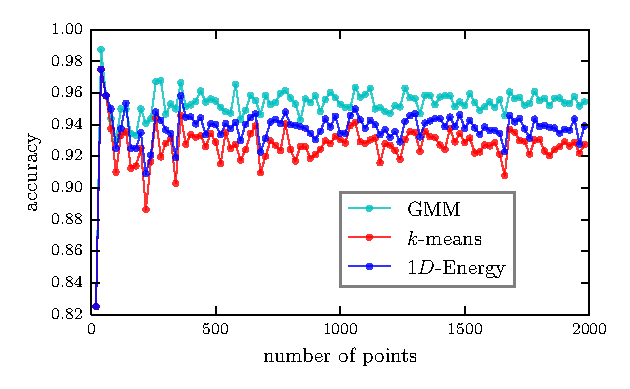
\includegraphics[width=\textwidth]{normal.pdf}\\[-1em]
(a)
\end{minipage}
\begin{minipage}{0.49\textwidth}
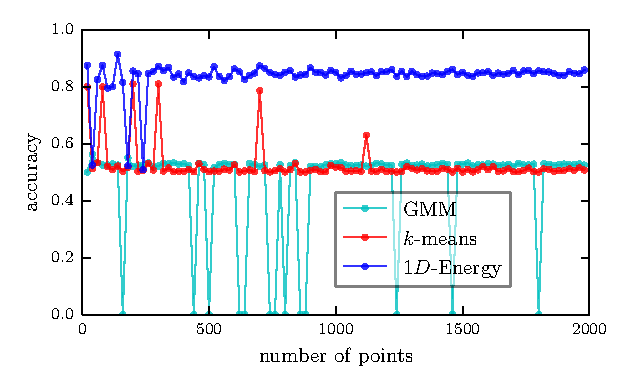
\includegraphics[width=\textwidth]{lognormal.pdf}\\[-1em]
(b)
\end{minipage}
\caption{
\label{fig:1d}
We cluster data using Algorithm~\ref{algo1d} ($1D$-Energy in the plots), 
GMM, and $k$-means. We use
\eqref{eq:accuracy} to evaluate cluster quality. Both clusters
have the same number of points, which are increased in each experiment.
(a) 
$x\sim \tfrac{1}{2}\left( \mathcal{N}(\mu_1,\sigma_1) +
\mathcal{N}(\mu_2,\sigma_2)  \right)$ with 
$\mu_1 = 0$,
$\mu_2 = 5$,
$\sigma_1 = 1$, and
$\sigma_2 = 2$.
(b) 
$x\sim \tfrac{1}{2}\left( e^{\mathcal{N}(\mu_1,\sigma_1)} +
e^{\mathcal{N}(\mu_2,\sigma_2)}  \right)$ with 
$\mu_1 = 0$,
$\mu_2 = -1.5$,
$\sigma_1 = 0.3$, and
$\sigma_2 = 1.5$.
}
\end{figure}




%%%%%%%%%%%%%%%%%%%%%%%%%%%%%%%%%%%%%%%%%%%%%%%%%%%%%%%%%%%%%%%%%%%%%%%%%%%%%%%
\section{Iterative Algorithm for Energy Clustering}
\label{sec:algo}

In this section we will introduce a new iterative algorithm to find a local
maximizer of \eqref{eq:qcqp2}, however, due to 
Proposition~\ref{th:kernel_kmeans} we can also find an approximate
solution by the well-known kernel $k$-means algorithm. Thus, to be
self-contained let us first recall kernel $k$-means algorithm in this
context.

\subsection{Kernel $\bm{k}$-Means Algorithm}

Consider this optimization problem as
written in the form \eqref{eq:max_prob},
\begin{equation}
\label{eq:maxQ}
\max_{\{ \C_1,\dotsc,\C_k \}} 
\bigg\{ Q = \sum_{j=1}^k \dfrac{Q_j}{n_j}  \bigg\},
\qquad Q_j = \sum_{x,y\in\C_j} \kk(x,y),
\end{equation}
where $Q_j$ represents the internal cost of cluster $\C_j$, and
$Q$ is the total cost where each cluster cost 
is weighted by the inverse
of the number of its elements. For a data point $x_i$ its cost
with cluster $\C_j$ is denoted by
\begin{equation}
\label{eq:costxij}
Q_j(x_i) \equiv \sum_{y\in\C_j} \kk(x_i, y) = 
G_{i \bullet} \cdot Z_{\bullet j}.
\end{equation}

Now for kernel $k$-means 
consider \eqref{eq:J} where we define
the function
\begin{equation}
\label{eq:Jell}
J^{(\ell)}(x_i) \equiv -\dfrac{2}{n_\ell} Q_\ell(x_i) + \dfrac{1}{n_\ell^2}
Q_\ell
\end{equation}
which represents the cost of $x_i$ with cluster $\C_\ell$. Thus,
one assigns point $x_i$ to the cluster $\C_{j^\star}$ according
to $j^\star = \argmin_\ell J^{(\ell)}(x_i)$, for $\ell = 1,\dotsc,k$.
This procedure is performed for every data point, and repeated until
convergence, i.e. until no new assignments are made.
The complete algorithm is shown in Algorithm~\ref{kmeans_algo}.
Although our formulation looks a little bit different than the standard
kernel $k$-means found in the literature \cite{Dhillon}, this is precisely
the same algorithm.

Notice that to compute the first term in \eqref{eq:Jell} requires
$\OO(n_\ell)$ operations, and although the second term requires
$\OO(n_\ell^2)$, it only needs to be computed once outside the loop through
data points. Therefore, the time complexity of this algorithm is
$\OO(n k \max_\ell n_\ell) = \OO(k n^2)$. If $G$ is sparse with 
$n'$ nonzero elements, this complexity can be further reduced
to $\OO(k n')$. 

\begin{algorithm}[H]
\vspace{.5em}
\begin{algorithmic}[1]
    \INPUT number of clusters $k$, Gram matrix $G$, initial label
    matrix $Z = Z_0$
    \OUTPUT label matrix $Z$ 
  \STATE Let $\bm{q} = (Q_1, \dotsc, Q_k)^\top$ 
            have the costs of each cluster, according to \eqref{eq:maxQ}
  \STATE Let $\bm{n} = (n_1,\dotsc,n_k)^\top$ have the number of elements
        in each cluster
  \REPEAT
    \FOR{ $i=1,\dotsc,n$}
        \STATE Let $j$ be such that $x_i \in \C_j$
        \STATE $j^\star \leftarrow \argmin_{\ell} J^{(\ell)}(x_i)$
            according to \eqref{eq:Jell}, for $\ell=1,2,\dots,k$
        \IF{ $j^\star \ne j$} 
            \STATE Move $x_i$ to $\C_{j^\star}$: $Z_{ij} \leftarrow 0$,
            $Z_{ij^\star} \leftarrow 1$
            \STATE Update $\bm{n}$: $n_j \leftarrow n_j - 1$,
                    $n_{j^\star} \leftarrow n_{j^\star} + 1$
            \STATE Update $\bm{q}$: $q_j \leftarrow q_j - 2Q_j(x_i)$, 
    $q_{j^\star} \leftarrow q_{j^\star} + 2Q_{j^\star}(x_i)$
    %    \ELSE
    %        \STATE Do nothing;
        \ENDIF
    \ENDFOR
  \UNTIL{convergence}
\end{algorithmic}
\caption{\label{kmeans_algo}
Kernel $k$-means algorithm 
to find an approximate solution to \eqref{eq:qcqp2}.}
\end{algorithm}


\subsection{Energy Cost Algorithm}

Now let us consider a different algorithm, which is based on computing
the difference in the energy cost when assigning a given data point to
a different partition.
Suppose we have a data point $x_i \in \mathcal{X}$
which is currently classified as being in cluster $\C_j$, yielding
a total cost function \eqref{eq:maxQ} denoted by $Q^{(j)}$.
Let us consider the change in the total cost by moving
$x_i$ to cluster $\C_\ell$. 
Denote the new total cost after moving $x_i$ to $\C_\ell$ by $Q^{(\ell)}$.
It is straightforward to see that
\begin{equation}
\label{eq:changeQ}
\begin{split}
\Delta Q^{j \to \ell}(x_i) &\equiv Q^{(\ell)} - Q^{(j)} \\ 
&= 
\dfrac{1}{n_j - 1}\left[ \dfrac{Q_j}{n_j} - 2 Q_j(x_i) \right]
- \dfrac{1}{n_\ell + 1}\left[ \dfrac{Q_\ell}{n_\ell} - 2 \big(Q_\ell(x_i) + 
\kk(x_i,x_i)\big) 
\right].
\end{split}
\end{equation}
Thus, if $\Delta Q^{j\to \ell}(x_i) > 0$ we get closer to a 
maximum of \eqref{eq:maxQ} by
moving $x_i$ to $\C_\ell$, otherwise we keep $x_i$ in $\C_j$. Based on
this we propose an algorithm where
the iterates are performed as follows.
We start with an initial configuration for the label matrix $Z$, 
then for each
point $x_i$ 
we compute the cost of moving it to another cluster,
$\Delta Q^{j\to \ell}(x_i)$ for 
$\ell=1,\dots,k$ with $\ell \ne j$. 
We then choose $j^\star = \argmax_\ell \Delta^{j \to \ell}(x_i)$.
If $\Delta Q^{j \to j^\star}(x_i) > 0$ 
we move $x_i$ to cluster $\C_{j^\star}$, otherwise 
we keep $x_i$ in its original cluster $\C_j$. We update $Z$ accordingly.
The process is repeated
until convergence, i.e. until no points are assigned to new clusters. 
This procedure is described in Algorithm~\ref{algo} below.

\begin{algorithm}[H]
\vspace{.5em}
\begin{algorithmic}[1]
    \INPUT number of clusters $k$, Gram matrix $G$, 
                initial label matrix $Z=Z_0$
    \OUTPUT label matrix $Z$
  \STATE Let $\bm{q} = (Q_1, \dotsc, Q_k)^\top$ 
            have the energy costs of each cluster, according to \eqref{eq:maxQ}
  \STATE Let $\bm{n} = (n_1,\dotsc,n_k)^\top$ have the number of elements
        in each cluster
  \REPEAT
    \FOR{ $i=1,\dotsc,n$}
        \STATE Let $j$ be such that $x_i \in \C_j$
        \STATE $j^\star \leftarrow \argmax_{\ell} \Delta Q^{j\to \ell}(x_i)$, 
            for $\ell=1,2,\dots,k$ and $\ell \ne j$ \label{stepmove}
        \IF{ $\Delta Q^{j \to j^\star}(x_i) > 0$ }
            \STATE Move $x_i$ to $\C_{j^\star}$: $Z_{ij} \leftarrow 0$,
            $Z_{ij^\star} \leftarrow 1$
            \STATE Update $\bm{n}$: $n_j \leftarrow n_j - 1$,
                    $n_{j^\star} \leftarrow n_{j^\star} + 1$
            \STATE Update $\bm{q}$: $q_j \leftarrow q_j - 2Q_j(x_i)$, 
    $q_{j^\star} \leftarrow q_{j^\star} + 2\left(Q_{j^\star}(x_i)+
    G_{ii}\right)$
    %    \ELSE
    %        \STATE Do nothing;
        \ENDIF
    \ENDFOR
  \UNTIL{convergence}
\end{algorithmic}
\caption{\label{algo}
Energy cost algorithm to find an approximate solution to \eqref{eq:qcqp2}.}
\end{algorithm}

Notice that computing $G$ requires $\OO( D n^2)$ operations, where 
$D$ is the dimension of each data point and $n$ is the data size. However,
both previous algorithms assume that $G$ is given. There are more efficient
methods to compute $G$, specially if it is sparse. We will not consider
this further, and just assume that $G$ is given.
The computation of each cluster cost
$Q_j$ has complexity $\OO(n_j^2)$, and overall to compute $\bm{q}$
we have $\OO(n_1^2+\dots + n_k^2) = \OO(k \max_j n_j^2)$. 
These operations, however, only need to be performed a single time. Now for
each point $x_i$ we need to compute $Q_j(x_i)$ once, which is
$\OO(n_j)$, and we need to compute $Q_\ell(x_i)$ for each $\ell\ne j$. 
The cost of computing 
\eqref{eq:costxij} is $\OO(n_j)$, thus the cost of step~$8$ in
Algorithm~\ref{algo} is $\OO(k \max_j n_j)$ for $j=1,\dotsc,k$.
For the 
entire dataset this gives a time-complexity
of $\OO(n k  \max_j n_j) =\OO(k n^2)$. This is the same cost as
in kernel $k$-means, Algorithm~\ref{kmeans_algo}. Again, if $G$ is sparse
this can be reduced to $\OO(k n')$, where $n'$ is the number of nonzero
entries of $G$.
In the numerical experiments below
we choose the initial $Z$ from the initialization 
procedure of $k$-means++ \cite{Vassilvitskii}. 


%%%%%%%%%%%%%%%%%%%%%%%%%%%%%%%%%%%%%%%%%%%%%%%%%%%%%%%%%%%%%%%%%%%%%%%%%%%%%%%
\section{Numerical Experiments}
\label{sec:numerics}

In the following experiments we fix the semimetric as $\rho(x,y) = \| x-y\|$,
with induced kernel 
\eqref{eq:kernel_semimetric}. We will compare Algorithm~\ref{algo} with
kernel $k$-means Algorithm~\ref{kmeans_algo}, and also with
standard $k$-means and GMM through the Expectation Maximization (EM) algorithm
as well. For synthetic data our measure of clustering performance
will be \eqref{eq:accuracy}. Moreover, for all the algorithms, we always
choose the initialization from $k$-means++ \cite{Vassilvitskii}.

We first consider clustering in high dimensions and analyze 
how the algorithms degrade as the number of dimensions increase, while
keeping the number of points in each cluster fixed. 
In Figure~\ref{fig:gauss}a we have data generated from normal 
distributions in 
$D$-dimensions:
\begin{equation}
\label{eq:gauss1}
\begin{split}
&x \sim \tfrac{1}{2}\left\{ 
\mathcal{N}(\mu_1,\Sigma_1) + \mathcal{N}(\mu_2, \Sigma_2)\right\}, \\
&\mu_1 = (\underbrace{0,\dotsc,0}_{\times D})^\top , \quad
\mu_2 = 0.7 \times (\underbrace{1,\dots,1}_{\times 10},
\underbrace{0,\dots,0}_{\times (D-10)})^\top, \quad
\Sigma_1 = \Sigma_2 = I_D.
\end{split}
\end{equation}
For each experiment we only keep signal in
$\mu_2$ in the first $10$
dimensions, and keep increasing the ambient dimension $D$. For each
data set, we run the algorithms $10$ times and pick the result with
the best objective function value.
In Figure~\ref{fig:gauss}a one sees that
GMM is not able to estimate the covariance matrix 
when the number
of dimensions exceeds the number of points in each cluster. 
One can see a slightly better performance of Algorithm~\ref{algo} compared
to the other ones.
In Figure~\ref{fig:gauss}b we have the same type of experiment but 
with 
\begin{equation}
\label{eq:gauss2}
\begin{split}
&x \sim \tfrac{1}{2}\left( 
\mathcal{N}(\mu_1,\Sigma_1) + \mathcal{N}(\mu_2, \Sigma_2)\right), \\
&\mu_1 = (\underbrace{0,\dotsc,0}_{\times D})^\top , \,
\mu_2 = 0.7 \times (\underbrace{1,\dots,1}_{\times 10},
\underbrace{0,\dots,0}_{\times (D-10)})^\top, \,
\Sigma_1 = I_D, \, 
\Sigma_2 = \left( \begin{smallmatrix} \tfrac{1}{2} I_{10} & 0 \\ 0 & I_{D-10}
\end{smallmatrix}\right). \quad
\end{split}
\end{equation}

\begin{figure}
\begin{minipage}{0.49\textwidth}
\centering
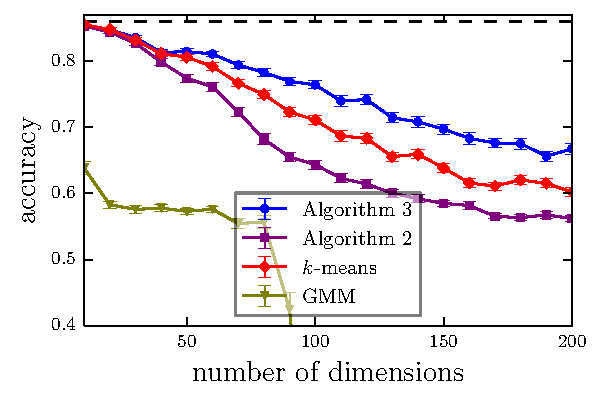
\includegraphics[width=1\textwidth]{gauss_dim.pdf}\\[-.8em]
(a)
\end{minipage}
\begin{minipage}{0.49\textwidth}
\centering
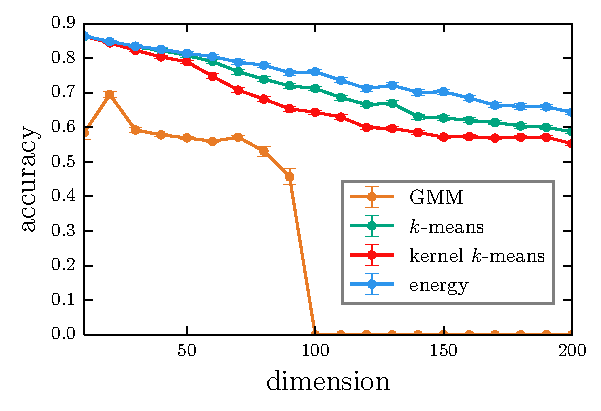
\includegraphics[width=1\textwidth]{gauss_cov.pdf}\\[-.8em]
(b)
\end{minipage}
\caption{
\label{fig:gauss}
Experiments where data is normally distributed.
(a) We keep $100$ points on each cluster
and increase the ambient dimension, as described in \eqref{eq:gauss1}. The blue
dots correspond to Algorithm~\ref{algo}, while
the red dots 
corresponds to Algorithm~\ref{kmeans_algo}.
(b) The same but with data following \eqref{eq:gauss2}.
In both experiments one notice a slightly better accuracy
of Algorithm~\ref{algo} compared to the other ones.
}
\end{figure}



In Figure~\ref{fig:unbalanced}a we consider how the previous algorithms
behave
for unbalanced clusters. We generate data as
\begin{equation}
\label{eq:gauss3}
\begin{split}
&x \sim  
\dfrac{n_1}{N} \mathcal{N}(\mu_1,\Sigma_1) + 
\dfrac{n_2}{N} \mathcal{N}(\mu_2, \Sigma_2), 
\quad \mu_1 = (0,0,0,0)^\top , \,
\mu_2 = 1.5\times (1,1,0,0)^\top, \\
&
\Sigma_1 = I_4, \quad
\Sigma_2 = \left( 
\begin{smallmatrix} 
1/2 & 0 & 0 & 0\\
0 & 1/2 & 0 & 0 \\
0 & 0 & 1 & 0 \\
0 & 0 & 0 & 1 
\end{smallmatrix}\right), \quad
n_1 = N - m, \quad  n_2 = N + m, \quad N=200,
\end{split}
\end{equation}
and we increase $m$, i.e. we make the clusters progressively more unbalanced.
As well-known, one an see that GMM
works well for unbalanced clusters, mostly because 
it is a soft clustering algorithm.
We can see that all the other kernel based methods
degrade more rapidly than GMM for
highly unbalanced clusters.
This is
unsurprising since Algorithms~\ref{algo}~and~\ref{kmeans_algo} both 
make hard assignments. Finally, Figure~\ref{fig:unbalanced}b considers
the same experiment as in Figure~\ref{fig:gauss}a but for lognormal
data. With $\rho(x,y) = \| x-y\|^{1/2}$ we even gain a slight improvement.
Energy statistics clustering outperforms all the other methods since
it is nonparametric.

\begin{figure}
\begin{minipage}{0.49\textwidth}
\centering
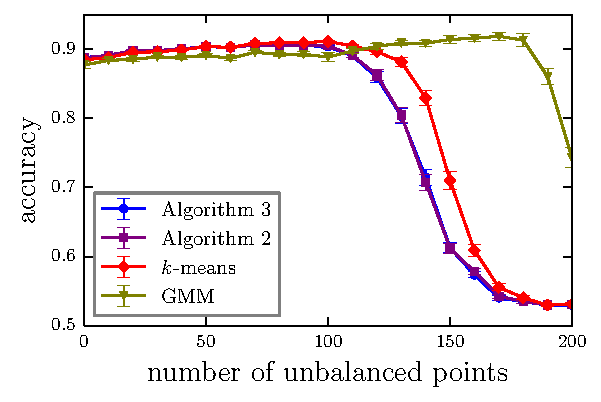
\includegraphics[width=1\textwidth]{gauss_pi.pdf}\\[-.8em]
(a)
\end{minipage}
\begin{minipage}{0.49\textwidth}
\centering
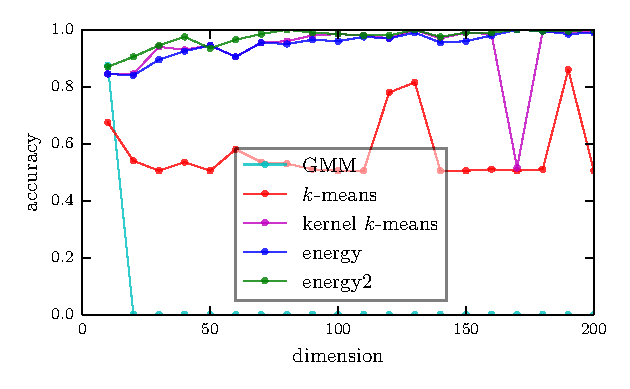
\includegraphics[width=1\textwidth]{loggauss_dim.pdf}\\[-.8em]
(b)
\end{minipage}
\caption{
\label{fig:unbalanced}
(a) Previous algorithms for unbalanced clusters, 
according to \eqref{eq:gauss3}.
(b) The same experiment as in Figure~\ref{fig:gauss}a but for lognormal
data as 
$x\sim \tfrac{1}{2}\left( e^{\mathcal{N}(\mu_1,\Sigma_1)} +
e^{\mathcal{N}(\mu_2,\Sigma_2)} \right)$ with
$\mu_1 = (0,\dotsc,0)^\top$,
$\mu_2 = 0.5\times(1,\dotsc,1,0,\dotsc,0)^\top$ with signal in $d=10$, 
$\Sigma_1 = 0.3 \times I_D$, and $\Sigma_2=I_D$. 
One see a clear advantage of
energy statistics clustering. The extra green line correspond
to $\rho(x,y) = \| x-y\|^{1/2}$.
}
\end{figure}


In Figure~\ref{fig:weird} we consider other types of data in two dimensions.
In each case we perform 10 experiments and compute the accuracy
based on the true labels. The plots show the average results of 10 runs
of each experiment (dots), and the maximum and minimum values as well (shaded
area). Although energy clustering is nonparametric, these datasets are
very specific so we can take advantage and make a suitable choice of
the semimetric $\rho$. This illustrates that energy clustering is also
flexible enough to incorporate prior information about the data.
In Figure~\ref{fig:weird}a we have parallel cigars from
\begin{equation}
\label{eq:cigar}
\begin{split}
&x \sim \tfrac{1}{2}\left( 
\mathcal{N}(\mu_1, \Sigma_1) + 
\mathcal{N}(\mu_2, \Sigma_2)
\right), \\
& \mu_1 = (0,0)^\top, \quad \mu_2 = (6.5, 0)^\top, \quad
\Sigma_1 = \Sigma_2 = \left( \begin{smallmatrix} 
1 & 0 \\ 0 & 20
\end{smallmatrix}\right)
\end{split}
\end{equation}
with $100$ points in each cluster. Notice that $k$-means is unable to
cluster this data, while energy clustering performs pretty much as well
as GMM, which is the optimal algorithm suited to this kind of data.
We used the semimetric $\rho(x,y) = \| x -  y\|^{1/2}$ in this case.
In Figure~\ref{fig:weird}b we generate two concentric circles with a small
gaussian noise. To make the semimetric a little bit more localized we
include a decaying exponential in the form:
\begin{equation}
\label{eq:rho_loc}
\rho(x,y) = \| x-y \|^2 e^{-\tfrac{1}{2}\| x-y \|}.
\end{equation}
Notice that energy clustering is able to cluster this data almost perfectly
in most cases.
In Figure~\ref{fig:weird}c we consider two spirals, also with a small
gaussian noise. Due to the geometry of the data
we consider
\begin{equation}
\label{eq:rho_sin}
\rho(x,y) = \| x - y\|^2 \theta \sin \left(  \tfrac{\| x-y \|}{\theta}\right),
\qquad \theta = 0.9.
\end{equation}
Again, energy clustering performs much better than $k$-means and GMM which
are unable to cluster this kind of dataset.


\begin{figure}
\begin{minipage}{0.33\textwidth}
\hspace{.7cm}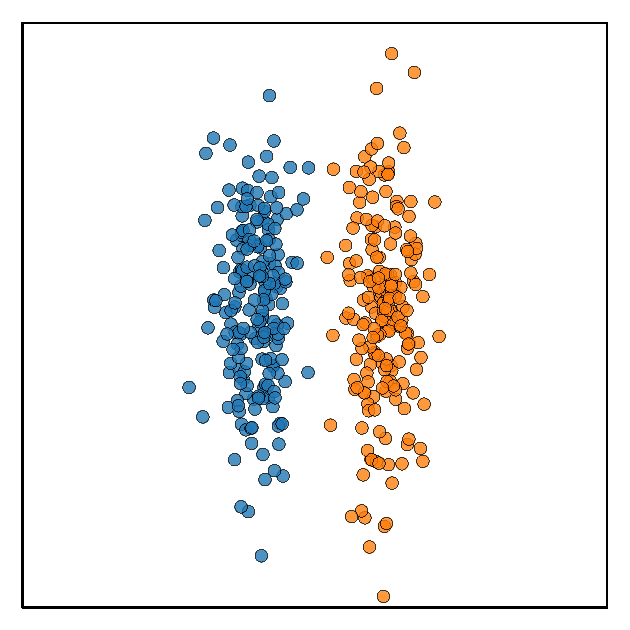
\includegraphics[width=.82\textwidth]{cigar_data.pdf}
\end{minipage}
\begin{minipage}{0.33\textwidth}
\hspace{.7cm}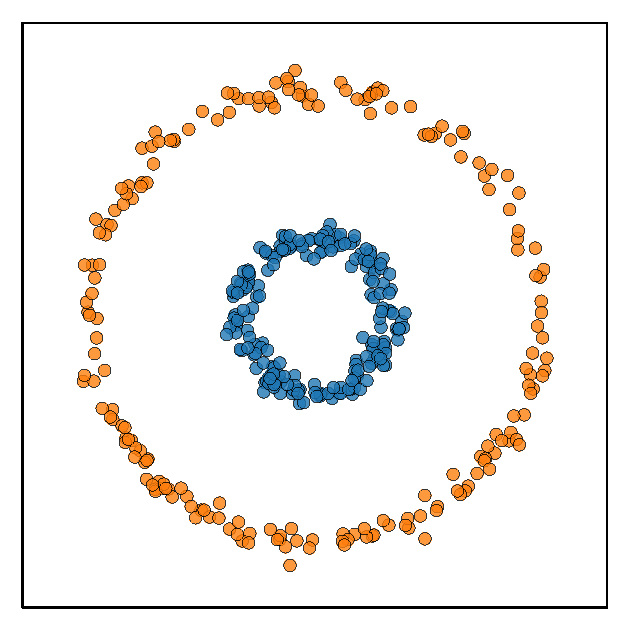
\includegraphics[width=.82\textwidth]{circles_data.pdf}
\end{minipage}
\begin{minipage}{0.33\textwidth}
\hspace{.7cm}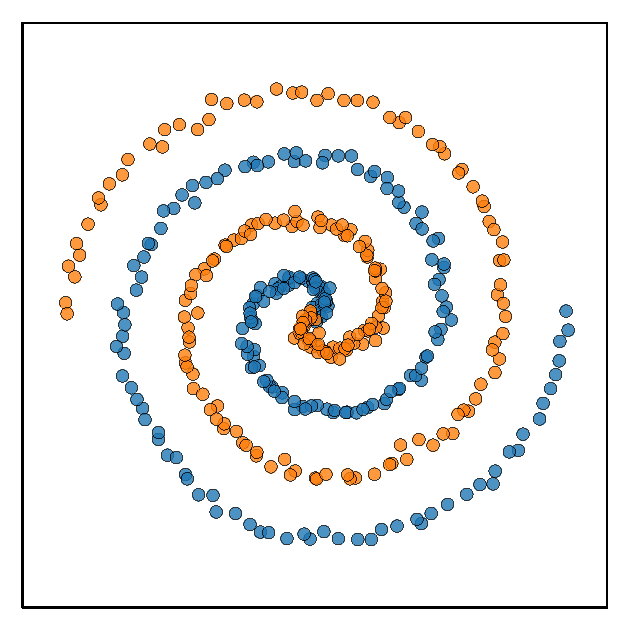
\includegraphics[width=.82\textwidth]{spirals_data.pdf}
\end{minipage}
\begin{minipage}{0.33\textwidth}
\centering
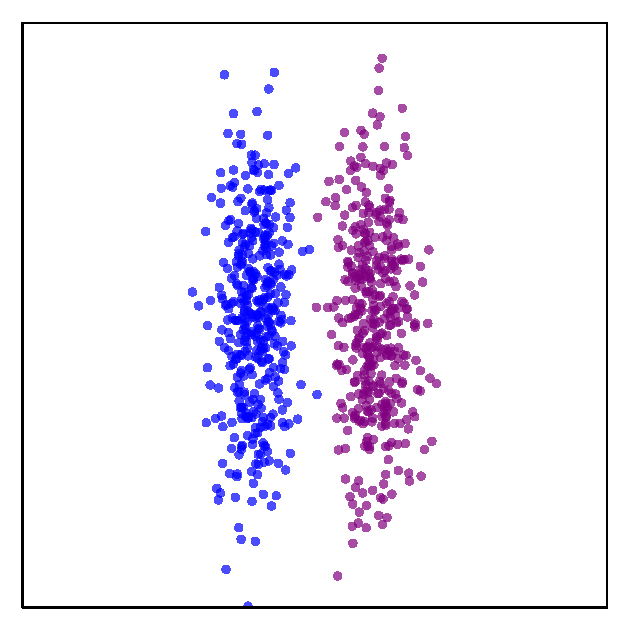
\includegraphics[width=\textwidth]{cigars.pdf}\\[-.8em]
(a)
\end{minipage}
\begin{minipage}{0.33\textwidth}
\centering
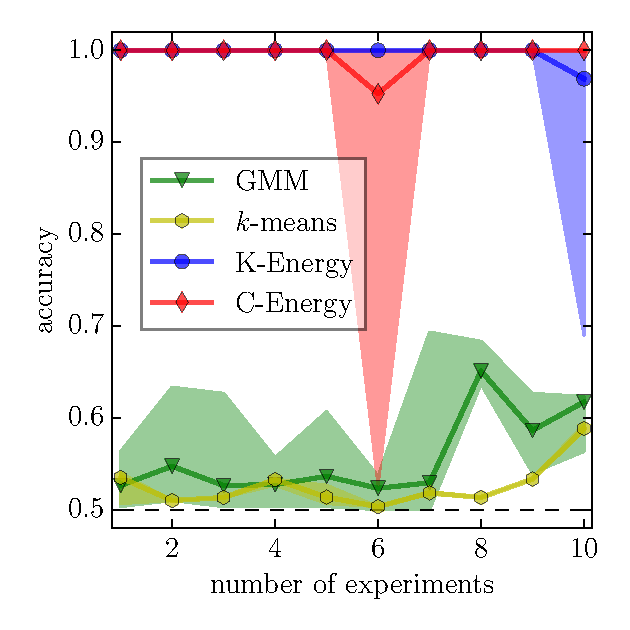
\includegraphics[width=\textwidth]{circles.pdf}\\[-.8em]
(b)
\end{minipage}
\begin{minipage}{0.33\textwidth}
\centering
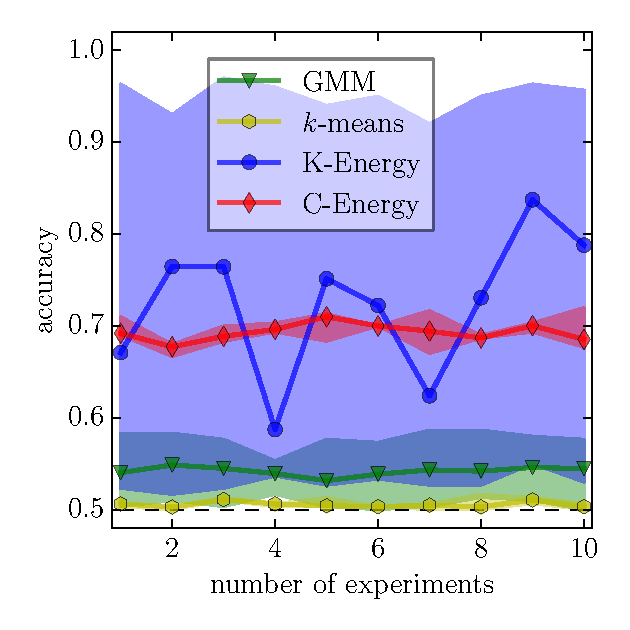
\includegraphics[width=\textwidth]{spirals.pdf}\\[-.8em]
(c)
\end{minipage}
\caption{
\label{fig:weird}
(a) Parallel cigars generated from \eqref{eq:cigar} with $100$ points
in each class. Use use energy clustering
with $\rho = \| x - y\|^{1/2}$. (b) Two concentric circles with $150$ points
in each class. We use the semimetric \eqref{eq:rho_loc}. 
(c) Two concentric spirals with
$150$ points in each class. We use the semimetric \eqref{eq:rho_sin}.
}
\end{figure}


\section{Conclusion}


\subsection*{Acknowledgements}
We thank \ldots


\bibliographystyle{unsrt}
\bibliography{biblio.bib}



\end{document}
